\documentclass[12pt, twoside]{article}
\usepackage[letterpaper, margin=1in, headsep=0.2in]{geometry}
\setlength{\headheight}{0.6in}
%\usepackage[english]{babel}
\usepackage[utf8]{inputenc}
\usepackage{microtype}
\usepackage{amsmath}
\usepackage{amssymb}
%\usepackage{amsfonts}
\usepackage{siunitx} %units in math. eg 20\milli\meter
\usepackage{yhmath} % for arcs, overparenth command
\usepackage{tikz} %graphics
\usetikzlibrary{quotes, angles}
\usepackage{graphicx} %consider setting \graphicspath{{images/}}
\usepackage{parskip} %no paragraph indent
\usepackage{enumitem}
\usepackage{multicol}
\usepackage{venndiagram}

\usepackage{fancyhdr}
\pagestyle{fancy}
\fancyhf{}
\renewcommand{\headrulewidth}{0pt} % disable the underline of the header
\raggedbottom
\hfuzz=2mm %suppresses overfull box warnings

\usepackage{hyperref}

\fancyhead[LE]{\thepage}
\fancyhead[RO]{\thepage \\ Name: \hspace{4cm} \,\\}
\fancyhead[LO]{BECA / Dr. Huson / Geometry\\*  Unit 4: Volume and polyhedra \\* 22 November 2022}

\begin{document}

\subsubsection*{4.10 Test: Solids, volume, and density \hfill HSA.CED.A1}
  \begin{enumerate}

\item Find the volume of a rectangular prism volume of water. Its length is $l=20$ feet, its height $h=12$ feet, and depth is $w=10$ feet. Start with the equation \\[0.5cm]
$V = l \times w \times h$
  \begin{flushright}
    \begin{tikzpicture}[scale=1.25]
      \draw [-, thick] (0,0)--(4,0)--(4,2)--(0,2)--cycle;
      \draw [-, thick] (0,2)--(0.5,2.75)--(4.5,2.75)--(4,2);
      \draw [-, thick] (4,0)--(4.5,0.75)--(4.5,2.75);
      \node at (4.75, 1.75){$12$};
      \node at (2, -0.25){$20$};
      \node at (4.5, 0.25){$10$};
    \end{tikzpicture}
  \end{flushright}

\item A parallelogram is shown on the $x$-$y$ plane having a base $b=4.25$ and height $h=7.0$. 
  \begin{multicols}{2}
    Find its area, showing the calculation.
      \begin{flushright}
      \begin{tikzpicture}[scale=.635]
        %\draw [help lines] (-1,-1) grid (9,6);
        \draw [thick, ->] (-1.2,0) -- (7.4,0) node [below right] {$x$};
        \draw [thick, ->] (0,-1.2)--(0,6.4) node [left] {$y$};
        \draw [<->, thick] (1.5,1)--(1.5,5);
        \draw [-, thick] (2,1)--(4.75,1)--(5.75,5)--(3,5)--cycle;
        \node at (3.5,1)[below]{$4.25$};
        \node at (1.5,3)[left]{$7.0$};
      \end{tikzpicture}
      \end{flushright}
  \end{multicols} 

\item Given the circle centered at $O$ with radius $r=3$. Leave answers in terms of $\pi$.
  \begin{multicols}{2}
    \begin{enumerate}
      \item Write down the length of the circle's diameter.
      \item Find the circumference of a circle. \vspace{1cm}
      \item Find the area of the circle.\vspace{1cm}
    \end{enumerate}
    \columnbreak
    \begin{flushright}
    \begin{tikzpicture}[scale=.635]
      \draw [help lines] (-5,-5) grid (5,5);
      \draw (0,0) circle [radius=3] node[below]{$O$};
      \draw [fill] (0,0) circle [radius=0.05];
    \end{tikzpicture}
  \end{flushright}
  \end{multicols} \vspace{1cm}

\newpage
\item Find the width of a rectangle with area $A=75$ and length $l=15$. Start with the form (use $w$ or $x$ for the unknown value): \\[0.5cm]
$A = l \times w = 75$
  \begin{flushright}
  \begin{tikzpicture}[scale=1, rotate=90]
    \draw [-, thick] (0,0)--(2,0)--(2,6)--(0,6)--cycle;
    \node at (-0.5, 3){$15$};
    \node at (1, -0.5){$?$};
    \node at (1, 3){$A=75$};
  \end{tikzpicture}
  \end{flushright}

\item The rectangular prism shown has a volume of $V=1815$ cubic centimeters. Its base measures $l=12.5$ cm by $w=8.8$ cm. \\[0.5cm]
Find its height in centimeters. Begin by writing the following formula with values substituted: \\[0.5cm]
$V = l \times w \times h = 1815$
\begin{flushright}
  \begin{tikzpicture}[scale=1]
    \draw [-, thick] (0,0)--(3,0)--(3,4)--(0,4)--cycle;
    \draw [-, thick] (0,4)--(0.5,4.75)--(3.5,4.75)--(3,4);
    \draw [-, thick] (3,0)--(3.5,0.75)--(3.5,4.75);
    \node at (3.75, 2.75){$h$};
    \node at (1.5, -0.25){$12.5$};
    \node at (4, 0.25){$8.8$};
  \end{tikzpicture}
\end{flushright}

\item Find the length of the base of a triangle with area $A=30$ and height $h=6 \frac{2}{3}$. Start with the form (use $b$ or $x$): \\[0.5cm]
$A = \frac{1}{2} \times b \times h = 30$
  \begin{flushright}
  \begin{tikzpicture}[scale=1.25]
    \draw [-, thick] (-1,0)--(3,0)--(2.5,3.5)--cycle;
    \draw[<->, dashed] (3.2,0)--(3.2,3.5);
    \node at (3.6, 1.5){$\displaystyle 6 \frac{2}{3}$};
    \node at (1, -0.5){$?$};
    \node at (1.5, 1){$A = 30$};
  \end{tikzpicture}
  \end{flushright}

\newpage
\subsubsection*{Model the situation with an equation starting with a labeling variable. \\ Do NOT solve! \hfill HSG.GMD.A3}

\item \emph{Worked example:} Find the radius of a circle with an area of 100.
\[A=\pi r^2=100\]

\item A sphere has a radius of 5 centimeters. Find the volume of the sphere. \vspace{2cm}

\item A large concrete post in the shape of a cylinder has a volume of 250 cubic feet. Its height is 12 feet. Find the radius of the base of the post. \vspace{2cm}

\item A prism has a base area of 40 square centimeters. Its volume is 300 cubic centimeters. Find the prism's height, $h$. \vspace{2cm}

\item The volume of a waffle cone having a \textbf{diameter} of 3 inches is 50 cubic inches. Find the cone's height. \vspace{2cm}

\item The volume of the Great Pyramid of Giza, the tomb of Pharoah Khufu, is approximately 2,500,000 cubic meters. It is 140 meters tall. Find the area of its base.  \vspace{2cm}

\item The smaller pyramid for his wife, Queen Meretites, has a square base with an area of 2500 square meters. Find the length of the side of its base, $s$.

\newpage
\subsubsection*{Apply the concept of density. Solve and state units. \hfill HSG.MG.A2}

\item A large bill board might be 20 feet high by 60 feet wide. If billboard paper costs approximately 25 cents per square foot, how much would the paper cost to cover such a billboard? \vspace{3cm}

\item Find the population density of Staten Island, New York (Richmond County) in people per square mile.
  \begin{multicols}{2}
  Population estimate July 1, 2019: 476,143\\[0.25cm]
  Land area in square miles: 58.37
  \begin{flushright}
    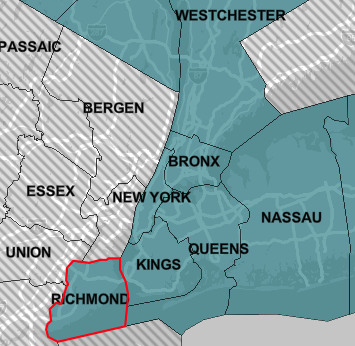
\includegraphics[width=7cm]{../graphics/04StatenIsland.png}\\
    Source: US Census (census.gov)
    %https://graspablemath.com/canvas?load=_0b517bab59c981c7
  \end{flushright}
  \end{multicols}

\item The American Eagle \emph{silver} coin is minted by the US Treasury. The one ounce coin has a radius of about $r=20$ millimeters and thickness $h=3$ mm. Given that the density of silver is $D = 0.0105$ grams per cubic millimeter, find the coin's volume and weight. \\[0.25cm]
  $\displaystyle V = \pi r^2 h$ and $W=VD$
    \begin{flushright}
      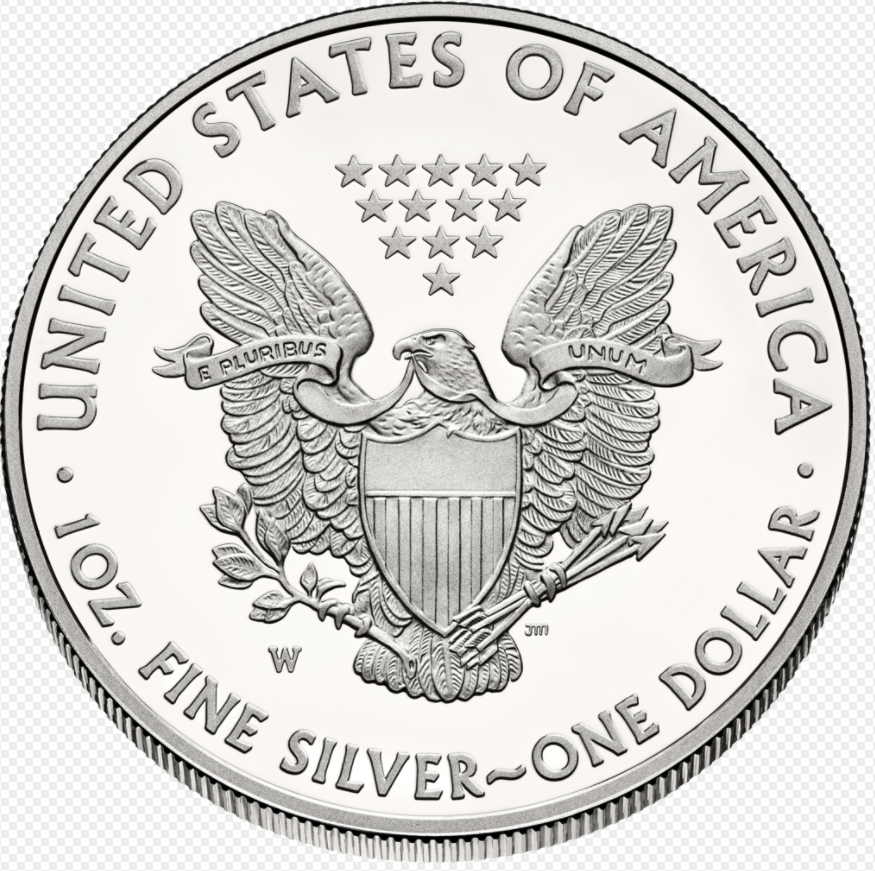
\includegraphics[width=5cm]{../graphics/04coin.png}
      %https://graspablemath.com/canvas?load=_845e39ea582acd9e
    \end{flushright}

\end{enumerate}
\end{document}